\documentclass[12pt, a4paper]{article}

\usepackage{import}
\usepackage{standalone}

\usepackage[top=4cm, right=2cm, bottom=2.7cm, left=2cm]{geometry}

\usepackage{wrapfig}
\usepackage{tabulary}
\usepackage{float}
\usepackage{pifont}
\usepackage{background}
\usepackage{tikz}


\pagestyle{empty}
\setlength{\parindent}{0pt}

\begin{document}
	\begin{minipage}{\textwidth}
		\section{Versnijden \hfill\small Bron: Bebras}
			Stel dat je een strook papier hebt van 16 cm lang en 1 cm hoog. Deze strook verdeel je in 16 kleine vierkantjes van 1 op 1 cm.
			\begin{figure}[H]
				\centering
				
\includegraphics[width=0.6\linewidth]{image1}
			\end{figure}
			Je plaatst de strook op een tafel en snijdt ze vervolgens in twee gelijke stukken. En daarna glijd je het rechterstuk 1 cm naar omhoog.
			\begin{figure}[H]
				\centering
				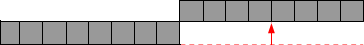
\includegraphics[width=0.6\linewidth]{image2}
			\end{figure}
			Daarna herhaal je dezelfde procedure voor elk van de beide stukken: je snijdt ze doormidden en glijdt het rechtergedeelte 1 cm naar omhoog.
			\begin{figure}[H]
				\centering
				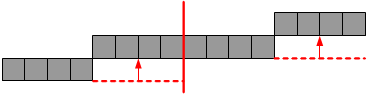
\includegraphics[width=0.6\linewidth]{image3}
			\end{figure}
			Tenslotte herhaal je dezelfde procedure voor deze 4 stukken en daarna nogmaals voor elk van de 8 stukken die je in de laatste stap hebt verkregen. \\
			
			Hoe ziet het eindresultaat er uit?
			
			\begin{table}[H]
				\centering
				\begin{tabulary}{\linewidth}{|C|C|C|}
					\hline
					\textbf{A} \vspace{0.2cm}
					
					
\includegraphics[width=0.9\linewidth]{option1}
					&
					\textbf{B} \vspace{0.2cm}
					
					
\includegraphics[width=0.9\linewidth]{option2}
					&
					\textbf{C} \vspace{0.4cm}
					
					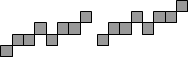
\includegraphics[width=0.9\linewidth]{option3}
					\\ \hline
					\textbf{D} \vspace{0.8cm}
					
					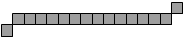
\includegraphics[width=0.9\linewidth]{option4}
					&
					\textbf{E} \vspace{0.6cm}
					
					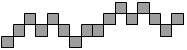
\includegraphics[width=0.9\linewidth]{option5}
					&
					\textbf{F} \vspace{0.2cm}
					
					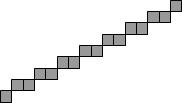
\includegraphics[width=0.9\linewidth]{option6}
					\\ \hline
				\end{tabulary}
			\end{table}
	\end{minipage} \\ \\
	
\end{document}	